\chapter{Avaliação da plataforma}

Nesse capítulo apresentamos um exemplo do uso do Comunidade.UnB em um ambiente
universitário e uma pesquisa com os alunos que fizeram uso do mesmo.
%
O estudo de caso foi baseado no uso do Comunidade.UnB, de diferentes, formas em
três disciplinas do curso de Engenharia de Software da FGA:
%
Desenho Industrial Assistido po Computador~\footnote{\url{%
https://wwwsec.serverweb.unb.br/matriculaweb/graduacao/disciplina.aspx?cod=199176}} (DIAC), 1º semestre;
%
Orientação a Objetos~\footnote{\url{%
https://wwwsec.serverweb.unb.br/matriculaweb/graduacao/disciplina.aspx?cod=195341}}
(OO), 3º semestre;
%
Manutenção e Evolução de Software~\footnote{\url{
https://wwwsec.serverweb.unb.br/matriculaweb/graduacao/disciplina.aspx?cod=206598}}
(MES), 7º semestre;
%
com a criação de uma comunidade para cada uma das disciplinas. Para a disciplina de
MES foram usadas ainda sub-comunidades para cada um dos projetos trabalhados nela.

\section{Uso do Noosfero em Disciplinas do Curso de Engenharia de Software}
\label{mes-unb}

O nível de uso da ferramenta variou de acordo com o semestre da disciplina. Na
disciplina de DIAC a comunidade foi utilizada mais como uma fonte de notícias
partindo do professor para os alunos. Os alunos foram encorajados ainda a publicar
as imagens de seus desenhos nas galerias de imagens de seus perfis, conforme
visto na figura \ref{imagem-diac}.

\begin{figure}[h!]
    \centering
		\rule{1cm}{1cm}
    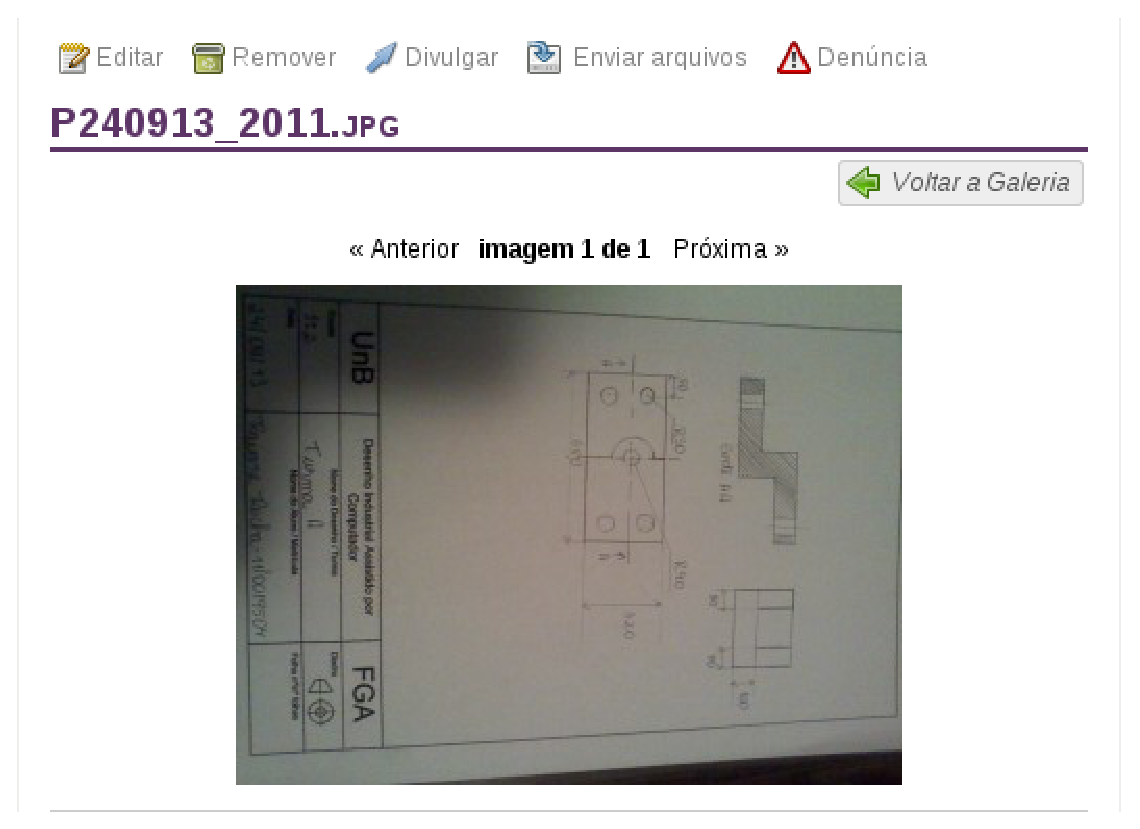
\includegraphics[keepaspectratio=true,scale=0.65]
      {figuras/imagem-diac.eps}
    \caption{Desenho desenvolvido na disciplina de DIAC:\newline
\url{http://comunidade.unb.br/raiane/galeria/p240913-2011.jpg}}
    \label{imagem-diac}
\end{figure}

A comunidade da disciplina de OO foi utilizada para  publicar os enunciados dos
trabalhos da disciplina e para receber os trabalhos dos alunos. Os enunciados
das provas das disciplinas também foram publicados na comunidade, assim como
seus gabaritos e revisões.
%
Na disciplina de MES, os alunos foram divididos em grupos para trabalhar com
manutenção e evolução de três projetos de software livre. Para isso foram
criadas sub-comunidades para cada um dos projetos:
%
(\textit{i}) Analizo;
(\textit{ii}) Noosfero;
e (\textit{iii}) Radar Parlamentar;
%
de forma que os progressos alcançados, materiais de estudo, referências
bibliográficas etc fossem publicadas em suas próprias sub-comunidades%
~\footnote{Uma sub-comunidade funciona como uma comunidade comum, porém
associada ao a uma comunidade ``mãe''.} (através do \textit{plugin} de
sub-organizações).

\begin{figure}[h!]
    \centering
    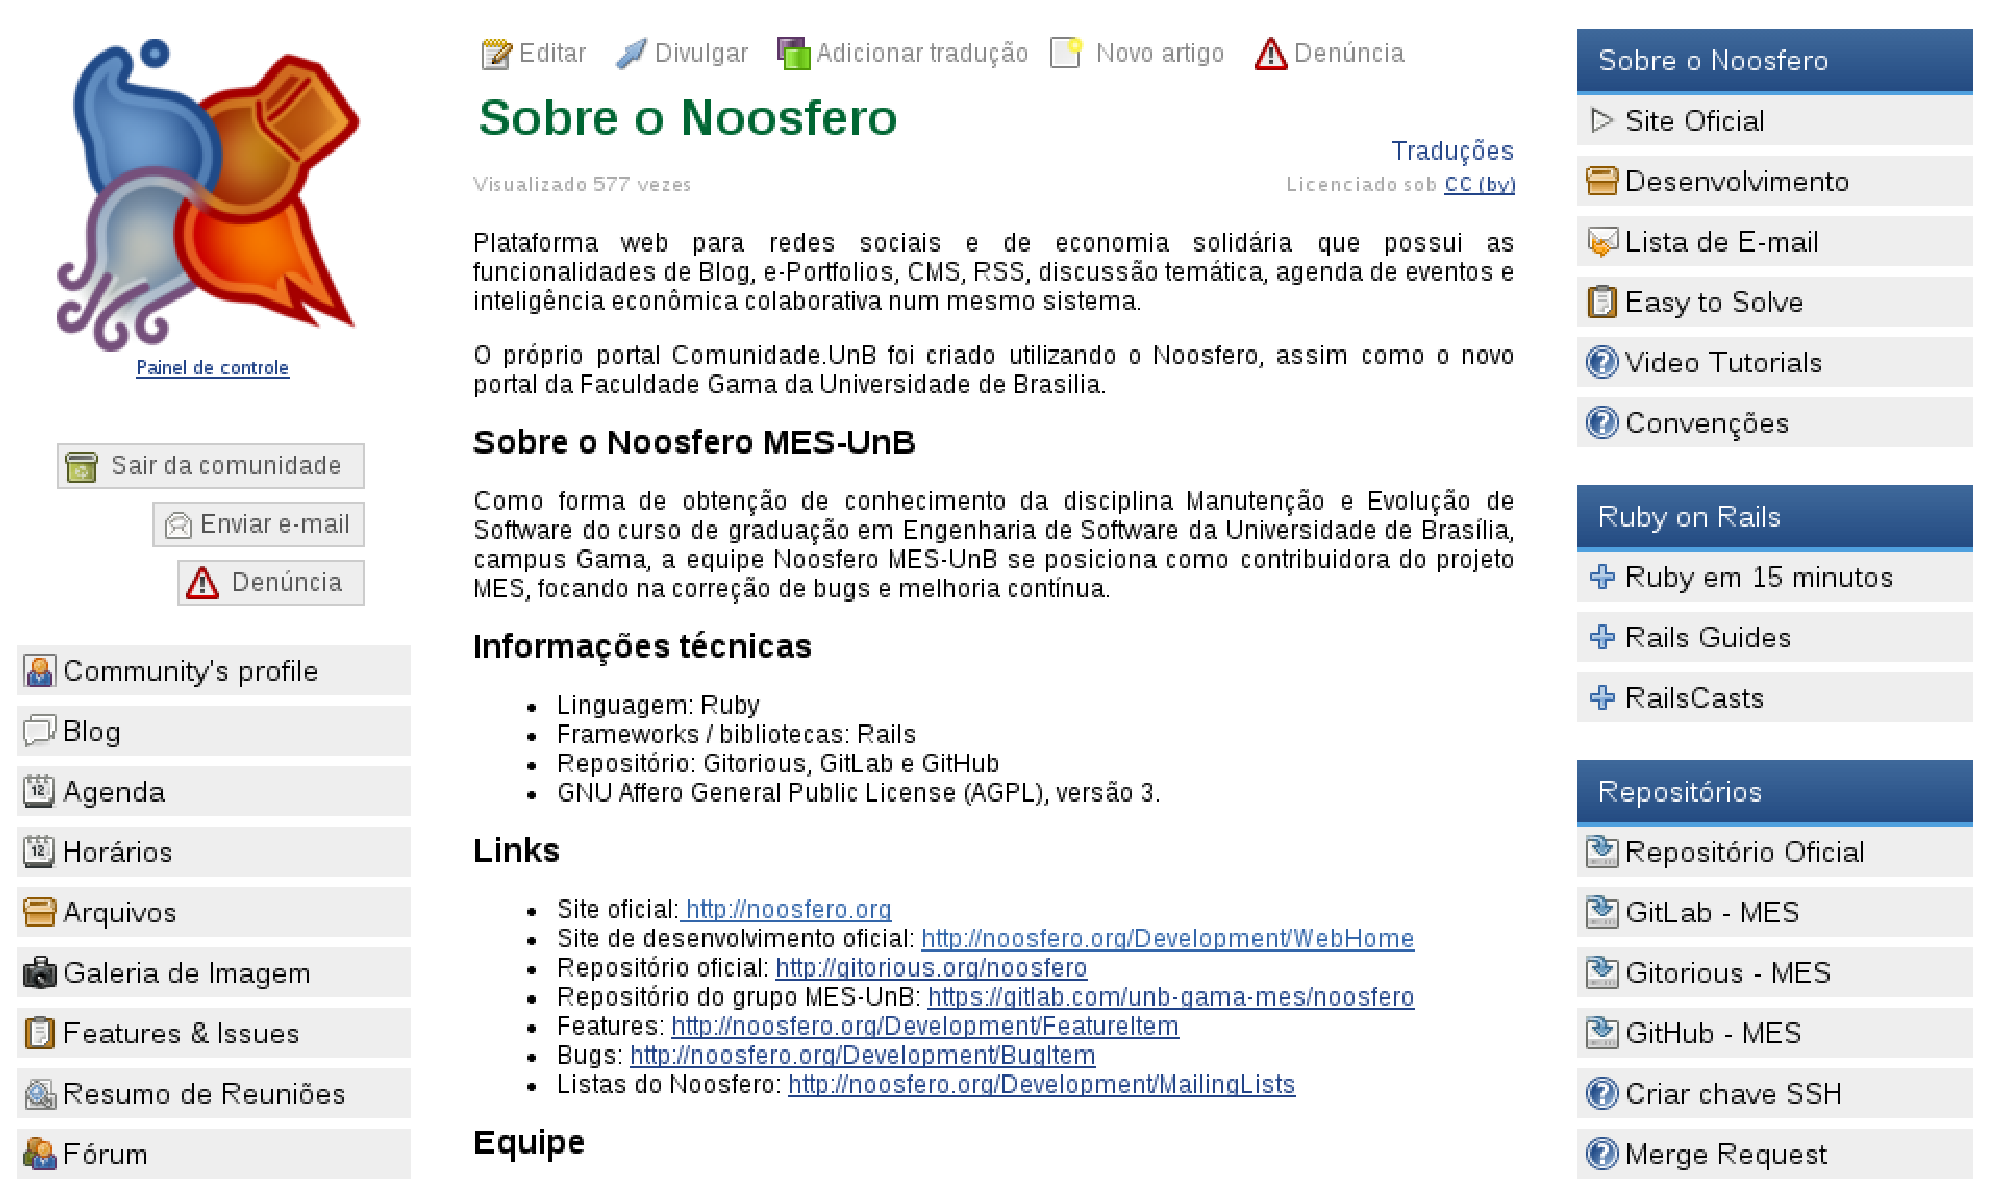
\includegraphics[keepaspectratio=true,scale=0.35]
      {figuras/Noosfero-MES.eps}
    \caption{Página inicial da sub-comunidade do projeto Noosfero da disciplina
    de MES:\newline \url{http://comunidade.unb.br/noosfero-mes-fga}}
    \label{mes-noosfero}
\end{figure}

A figura \ref{mes-noosfero} apresenta a página inicial,  da sub-comunidade do
time que colaborou com o Noosfero. Notamos que, conforme aumentava o semestre da
disciplina, e consequentemente a maturidade intelectual de seus alunos, o nível
do uso das funcionalidades de CMS do Noosfero, como a adição de blocos
laterais personalizados e a criação de conteúdos diversos, aumentou.

\section{Pesquisa com os usuários}

No mês de Dezembro de 2013 realizamos uma pesquisa junto aos alunos das três
disciplinas sobre o uso de uma rede social associada à marca da universidade
e sobre o nível de adequação do Noosfero para ser a plataforma adotada para
implantar essa rede.
%
Foi criado um questionário com cinco questões objetivas com a opção de
justificativa para as respostas.
%
Nesta seção apresentamos as questões elaboradas e as respostas coletadas
através da ferramenta \textit{Google Drive}.

\subsection*{Questão 01: Qual o seu semestre?}

A primeira pergunta tinha como objetivo levantar qual o semestre dos alunos
a responder o questionário e assim possivelmente associar as respostas
ao nível de maturidade dos alunos e ao tipo de uso que estes fizeram da rede.
%
A Figura \ref{response:p0} apresenta o resultado das pergutas. Podemos perceber
uma distribuição com mais alunos no início do curso e no final.
